Let \(M_i(t)=\mathbb{E}\{N_i(t)\}\) denote the mean cumulative function
(MCF) of \(N_i(t)\). The Nelson-Aalen estimator \citep{nelson2003siam}
are widely utilized in exploring the trend of recurrent event data. We
may use the \texttt{mcf()} function and the associated \texttt{plot()}
method provided by the \pkg{reda} package to visualize MCF estimates
stratified by whether the patients receive chemotherapy as follows.
Terminal events are ignored here for ease of illustration.

\begin{Shaded}
\begin{Highlighting}[]
\NormalTok{re\_mcf \textless{}{-}}\StringTok{ }\KeywordTok{mcf}\NormalTok{(}\KeywordTok{Recur}\NormalTok{(t.stop, id, event) }\OperatorTok{\textasciitilde{}}\StringTok{ }\NormalTok{chemo,}
              \DataTypeTok{data =}\NormalTok{ readmission)}
\KeywordTok{plot}\NormalTok{(re\_mcf, }\DataTypeTok{conf.int =} \OtherTok{TRUE}\NormalTok{, }\DataTypeTok{lty =} \DecValTok{1}\OperatorTok{:}\DecValTok{2}\NormalTok{) }\OperatorTok{+}
\StringTok{    }\NormalTok{ggplot2}\OperatorTok{::}\KeywordTok{theme}\NormalTok{(}\DataTypeTok{legend.position =} \StringTok{"bottom"}\NormalTok{)}
\end{Highlighting}
\end{Shaded}

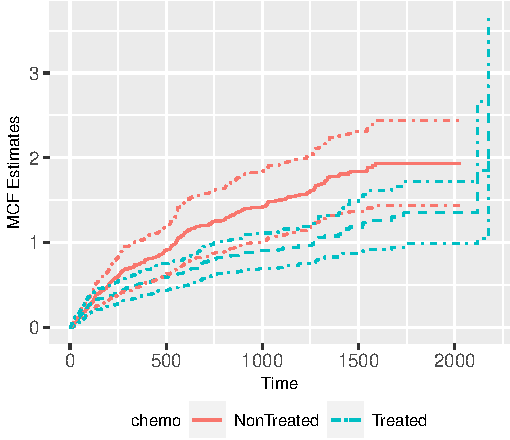
\includegraphics{reda-mcf_files/figure-latex/plot-sampleMcf-1.pdf}

The \texttt{plot()} method returns a \texttt{ggplot2} object
\citep{hadley2016ggplot2} so that users may further customize the plot
easily.

Furthermore, we may compare the MCF estimates using pseudo-score tests
\citep{cook1996biometrics} as follows:

\begin{Shaded}
\begin{Highlighting}[]
\KeywordTok{mcfDiff.test}\NormalTok{(re\_mcf)}
\end{Highlighting}
\end{Shaded}

\begin{verbatim}
Two-Sample Pseudo-Score Tests:
                Statistic Variance  Chisq DF Pr(>Chisq)  
Constant Weight     49.36   417.27   5.84  1      0.016 *
Linear Weight       38.08   264.06   5.49  1      0.019 *
---
Signif. codes:  
0 '***' 0.001 '**' 0.01 '*' 0.05 '.' 0.1 ' ' 1

Variance Estimator: robust 
\end{verbatim}
